% Samuel Emperador: filtrado y validación de municipios PDET (scripts/01_validate_mgn.py)
\section{Filtrado y validación de municipios PDET}\label{sec:validacion}

\textit{Responsable: Samuel Emperador. Script: \path{scripts/01_validate_mgn.py}.}

\subsection{Objetivo}

Antes de preparar y cargar los municipios hay que comprobar que la capa del MGN y la lista oficial PDET son coherentes entre sí: que cada uno de los 170 municipios PDET existe en el MGN con un código DIVIPOLA correcto, que ningún código está repetido y que las geometrías sirven para MongoDB. El script solo verifica y reporta; no modifica la capa ni repara geometrías (eso lo hace \path{02_prepare_municipalities.py}).

\subsection{Método}

\begin{enumerate}
  \item Lee el manifiesto de la descarga y se detiene (salida 2) si no acredita la capa nacional: sin manifiesto, \f{status} distinto de \f{complete}, capa ausente o SHA256 distinto del declarado.
  \item Lee la capa (GeoPackage, EPSG:4686) y la hoja \f{Hoja1} de \f{MunicipiosPDET.xlsx}.
  \item Normaliza los códigos con \f{zfill\_digits} del contrato: \f{MPIO\_CDPMP} y \f{Código DANE Municipio} a 5 dígitos (5031 $\rightarrow$ 05031), \f{DPTO\_CCDGO} a 2.
  \item Revisa la capa, la lista y el cruce por código (tabla~\ref{tab:verificaciones}). Cada geometría se clasifica como nula, vacía, no poligonal o inválida; para las inválidas se guarda el motivo de \f{shapely.explain\_validity}.
  \item Compara los nombres solo como información, separando las diferencias que son únicamente de tildes.
  \item Escribe tres salidas en \path{outputs/}: \f{mgn\_validation\_report.json} (resultado de cada verificación y \f{status} \f{valid}, \f{invalid} o \f{blocked\_no\_layer}), \f{mgn\_validation\_summary.md} y \f{pdet\_mgn\_crosswalk.csv} (una fila por municipio PDET).
\end{enumerate}

Una verificación es \emph{bloqueante} si su falla impide cargar los municipios. Las geometrías inválidas fuera de los PDET y las diferencias de nombre solo generan aviso. El código de salida es 0 si todas las bloqueantes pasan y 1 si alguna falla, así que los scripts siguientes (o quien los corra) pueden leer \f{status} antes de preparar o cargar.

\subsection{Resultados}

El reporte vigente fue generado por Miguel el 9 de noviembre de 2026 a las 07:27:37 (hora de Bogotá) sobre la capa de 1122 municipios que produce \path{01_download_mgn.py}. Reproduce el resultado inicial documentado por Samuel el 8 de noviembre: \textbf{\f{valid}}, 19 de 20 verificaciones en OK y un aviso informativo.

\begin{table}[htbp]
\centering\small
\caption{Verificaciones de \protect\path{01_validate_mgn.py} sobre la capa real. B: bloqueante.}\label{tab:verificaciones}
\begin{tabularx}{\textwidth}{@{}r L c l@{}}
\toprule
\# & Verificación & B & Resultado \\
\midrule
1 & Campos obligatorios del MGN (\f{MPIO\_CDPMP}, \f{MPIO\_CNMBR}, \f{MPIO\_NAREA}, \f{DPTO\_CCDGO}) & sí & OK \\
2 & Capa nacional con 1122 municipios & sí & OK: 1122 \\
3 & CRS EPSG:4686 & sí & OK \\
4 & \f{MPIO\_CDPMP} es DIVIPOLA de 5 dígitos & sí & OK: 0 errores \\
5 & Prefijo de \f{MPIO\_CDPMP} = \f{DPTO\_CCDGO} & sí & OK: 0 errores \\
6 & Sufijo de \f{MPIO\_CDPMP} = \f{MPIO\_CCDGO} & sí & OK: 0 errores \\
7 & Sin códigos repetidos en el MGN & sí & OK: 0 \\
8 & \f{MPIO\_NAREA} numérica y positiva & sí & OK \\
9 & Geometrías válidas en el MGN & no & OK: 0 inválidas \\
10 & Vértices dentro de la ventana lon/lat de Colombia & sí & OK \\
11 & Lista PDET con 170 filas & sí & OK: 170 \\
12 & Códigos PDET numéricos & sí & OK \\
13 & Sin códigos repetidos en la lista PDET & sí & OK: 0 \\
14 & 16 subregiones PDET & sí & OK: 16 \\
15 & Prefijo del código PDET = departamento del Excel & sí & OK \\
16 & Todos los municipios PDET están en el MGN & sí & OK: 0 faltantes \\
17 & Departamento del Excel = \f{DPTO\_CCDGO} del MGN & sí & OK: 0 \\
18 & Geometrías de los 170 PDET válidas & sí & OK: 0 inválidas \\
19 & Nombres iguales entre Excel y MGN & no & Aviso: 15 distintos \\
20 & Cruce completo de 170 municipios PDET & sí & OK: 170 \\
\bottomrule
\end{tabularx}
\end{table}

Los 170 municipios PDET cruzan con el MGN: no falta ninguno, no hay códigos repetidos en ninguna de las dos fuentes y los departamentos coinciden. Las 1122 geometrías son \f{MultiPolygon} válidas, ninguna nula o vacía, y todas caen en la ventana de Colombia (un control para detectar ejes latitud/longitud invertidos, sin certificar por sí solo el CRS). El área MGN de los 170 municipios suma 389\,182~km\textsuperscript{2}. La figura~\ref{fig:mapa-pdet} muestra el resultado del cruce.

\begin{figure}[htbp]
\centering
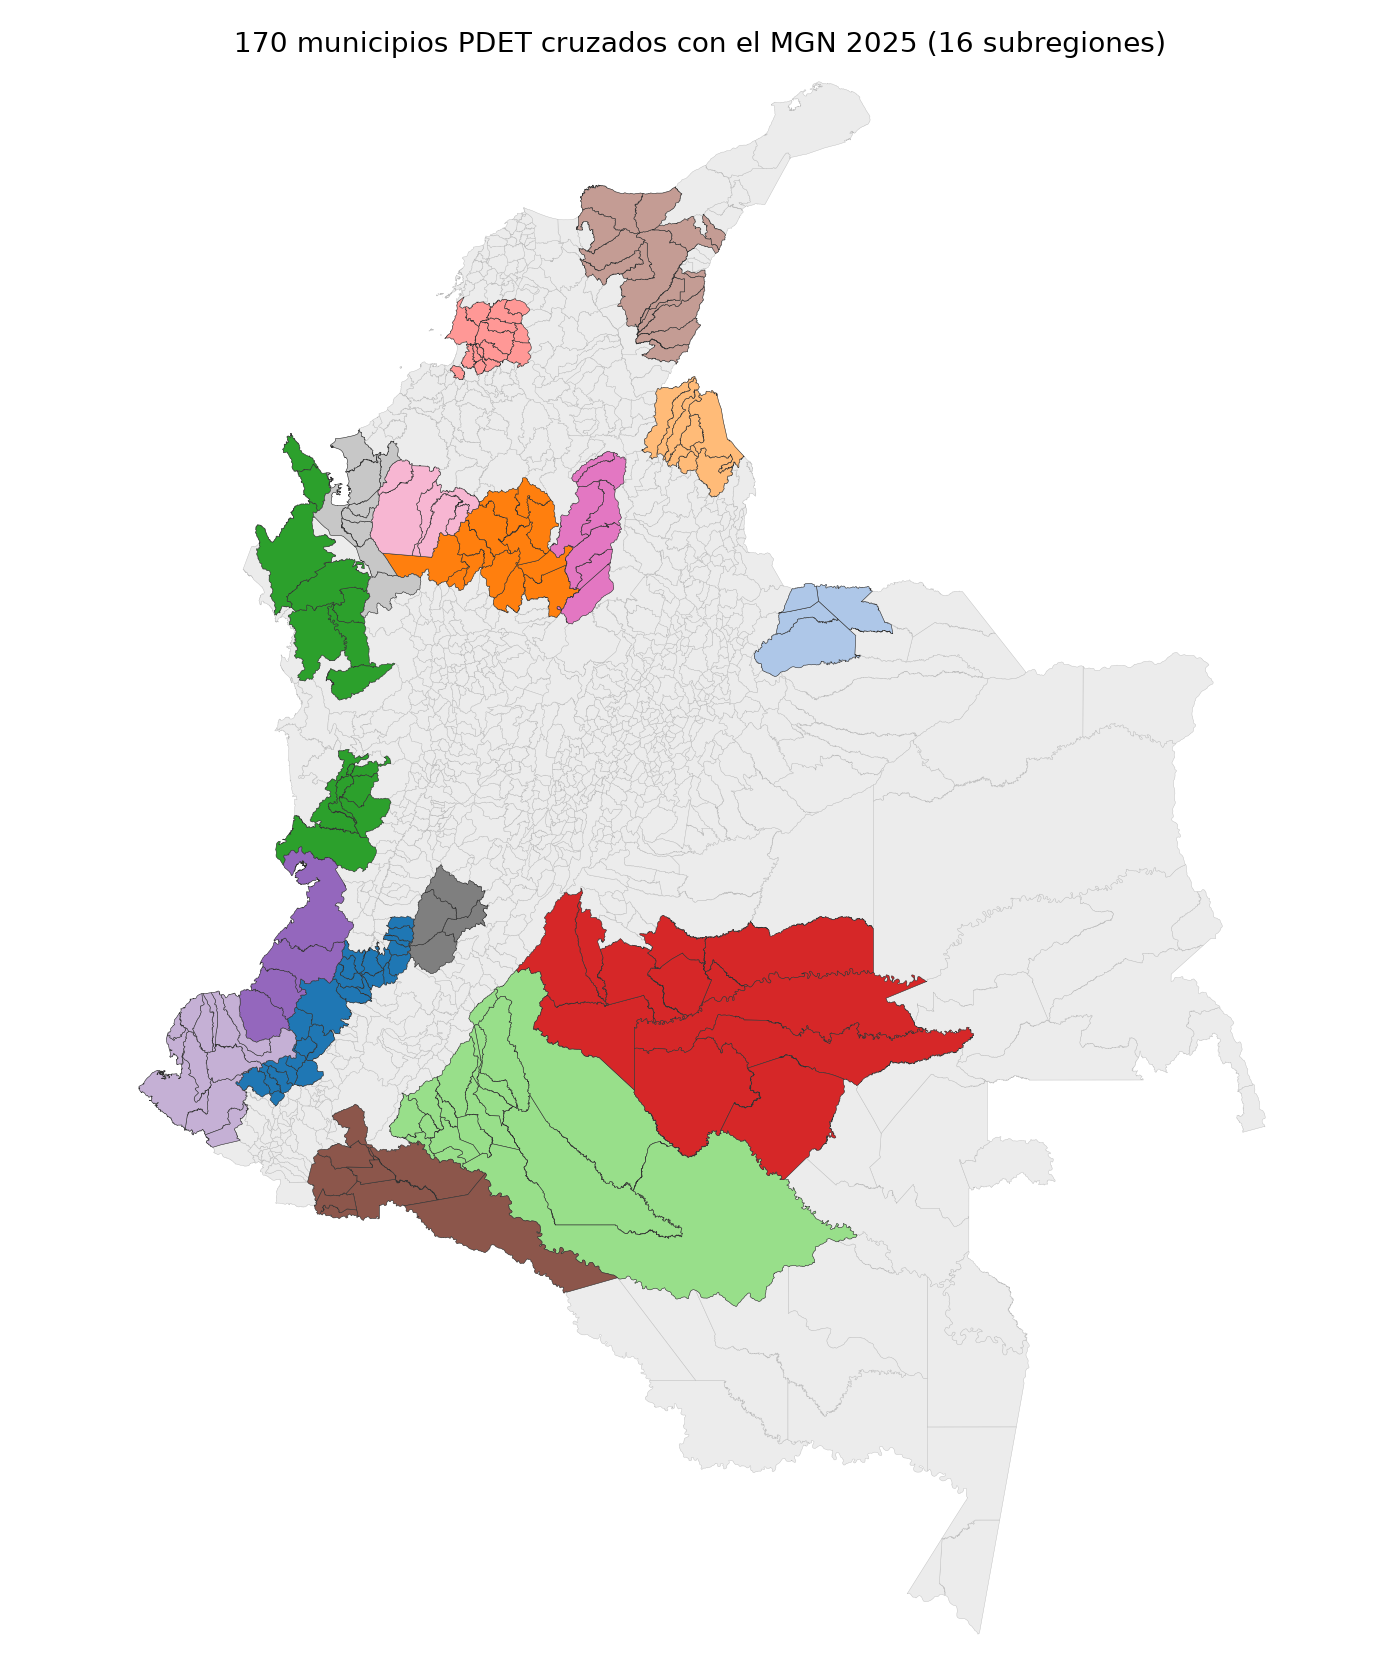
\includegraphics[width=0.62\textwidth]{figuras/mapa_pdet_validacion.png}
\caption{Municipios PDET cruzados con la capa MGN 2025; el color distingue la subregión. Generado con \protect\path{docs/delivery2/figuras/build_mapa_pdet.py} a partir de \f{pdet\_mgn\_crosswalk.csv}.}\label{fig:mapa-pdet}
\end{figure}

El único aviso son 15 nombres escritos distinto en el Excel y en el MGN (tabla~\ref{tab:nombres}): 9 difieren solo en tildes y 6 usan otra forma oficial del nombre. Ninguno afecta el cruce, que es por código, y la cifra coincide con \f{name\_mismatches} del reporte de preparación. Los documentos de \f{municipalities} usan el nombre del MGN.

\begin{table}[htbp]
\centering\small
\caption{Nombres distintos entre \f{MunicipiosPDET.xlsx} y el MGN 2025.}\label{tab:nombres}
\begin{tabularx}{\textwidth}{@{}l L L l@{}}
\toprule
Código & Excel & MGN & Tipo \\
\midrule
19548 & PIENDAMÓ & PIENDAMÓ - TUNÍA & forma oficial \\
50711 & VISTA HERMOSA & VISTAHERMOSA & forma oficial \\
70523 & SAN ANTONIO DE PALMITO & PALMITO & forma oficial \\
70823 & TOLÚ VIEJO & SAN JOSÉ DE TOLUVIEJO & forma oficial \\
19418 & LÓPEZ & LÓPEZ DE MICAY & forma oficial \\
86573 & LEGUÍZAMO & PUERTO LEGUÍZAMO & forma oficial \\
19821 & TORIBIO & TORIBÍO & tildes \\
27099 & BOJAYA & BOJAYÁ & tildes \\
27150 & CARMEN DEL DARIEN & CARMEN DEL DARIÉN & tildes \\
18256 & EL PAUJIL & EL PAUJÍL & tildes \\
70204 & COLOSO & COLOSÓ & tildes \\
52427 & MAGÜI & MAGÜÍ & tildes \\
52835 & SAN ANDRES DE TUMACO & SAN ANDRÉS DE TUMACO & tildes \\
23682 & SAN JOSE DE URE & SAN JOSÉ DE URÉ & tildes \\
05665 & SAN PEDRO DE URABA & SAN PEDRO DE URABÁ & tildes \\
\bottomrule
\end{tabularx}
\end{table}

\subsection{Pruebas del validador}

Como la capa real no tiene errores, cada verificación se probó también con figuras sintéticas (\f{python} \path{scripts/01_validate_mgn.py} \f{--self-check}, 19/19): municipio PDET ausente del MGN, código repetido en cada fuente, prefijo de departamento distinto, código no numérico, polígono autointersecado (falla dentro de los PDET y solo avisa fuera de ellos), punto en lugar de polígono, ejes invertidos, CRS EPSG:3857, capa incompleta, campo obligatorio faltante, y manifiesto ausente o bloqueado (salida 2).

\subsection{Observaciones}

\begin{itemize}
  \item El cambio de \f{timeStamp} que bloqueaba la comparación binaria ya se resuelve mediante \f{content\_sha256}, conservando los bytes originales. El manifiesto vigente registra coincidencia por contenido de las seis páginas (sección~\ref{sec:descarga}).
  \item El SHA256 del GeoPackage puede cambiar entre escrituras por sus metadatos; el GeoJSONL preparado sí sale idéntico. Por eso el validador compara la capa con el manifiesto de la misma corrida.
\end{itemize}
